\chapter{Introduction}
\label{ch:introduction}

Dimensionality reduction is one of the key research areas in the field of machine learning. As real world data sets are usually of high dimensionality, such as ..., methods to reduce this dimensionality are sought to alleviate the problems arising when dealing with high dimensional data. 

At present, much of the data being produced, gathered and analyzed is very high dimensional. As a consequence, several challenges arise when analyses are being performed on these vast amounts of high dimensional data.
At present, 

Several problems arise when dealing with high dimensional data:
- distances between pairs of points become less distinguished as dimensionality of the space increases \cite{on_the_surprising_behavior_of_distance_metrics}.
- The volume of a space grows exponentially along with the number of dimensions. This leads to even large data sets appearing sparse in the feature space. Efficient sampling requires a lot of points
- algorithms depend on dimensionality of the data being processed and large computational costs are accrued, especially sampling becomes
- need for more training data, k-means example \cite[p.~263]{understanding_machine_learning}
- algorithm complexity depends on the dimensionality of data being processed, large costs are accrued
- from a more practical perspective, high dimensional data by itself is hard to directly reason about and difficult to visualize in any meaningful sense
- In literature, problems arising from high dimensionality are collectively referred to as the \textit{curse of dimensionality}.
To tackle these problems associated with high dimensional data, reduction of the dimensionality of data is sought through various means of feature selection and feature extraction. Feature selection is ..., whereas feature extraction ... . In this work we focus on purely unsupervised feature extraction through 

Fortunately, the so called manifold hypothesis \cite{manifold_hypothesis} often holds for real world data sets. The manifold hypothesis posits that the high dimensional data in question lies near a much lower dimensional manifold. As an example, take This in turn implies that learning  

This, together with the classical Johnson-Lindenstrauss lemma \cite{johnson_lindenstrauss}, which gives bounds to the error 

The manifold assumption and manifold learning. In general, dimensionality reduction aims to preserve as much information of the underlying data as possible. Several different methods for dimensionality reduction have been developed over the years. Arguably the most well known and applied method in practice is Principal Component Analysis (PCA), developed independently by ... \cite{pca_1} and ... \cite{pca_2} for the study of ... . Although very efficient to compute and easy to reason about, PCA however suffers from a few drawbacks, making it not ideal for data visualization purposes. the fact that it only aims to maximize the variance... thus local structure of the data is poorly preserved. On the other hand, methods that aim to preserve local structure of data typically suffer from the curse of dimensionality in several ways, such as ... .

Dimensionality reduction is a tool commonly used in disciplines such as ... for visualization of high dimensional data as 2 or 3 dimensional scatter plots. 

In exploratory data analysis, visualization of the characteristics of data sets plays a key role.

In this work a method for improving the applicability of parametric t-SNE is proposed. In the proposed method a generative model in the form of a Variational Autoencoder is first trained and subsequently used to produce training data for the parametric t-SNE embedding. The benefits of this procedure are severalfold: . Further, each of these benefits are experimentally demonstrated on a variety of data sets, both quantitatively and qualitatively.

The structure of this thesis is as follows. In Chapter~\ref{ch:background_and_related_work} the relevant background and related work to the contribution of this thesis is covered to give context to an audience not previously familiar with variational autoencoders or the t-SNE method for dimensionality reduction. The chapter is organized into two main sections, one that builds up to the theory and recent advances in variational autoencoders from the introduction of neural networks, and the other section presents the development of t-SNE up to its parametrization with neural networks.

The method developed for this thesis is presented in Chapter~\ref{ch:method}. The proposed learning and inference algorithms are presented, together with discussion on extensions and further variations. In addition, relevant implementation details for the application built to produce the results for the experiments chapter are briefly covered.

In Chapter~\ref{ch:experiments} the proposed method is tested experimentally for different properties presented in the previous chapter, as well as compared with existing methods. The experiments chapter includes descriptions for the various data sets being used and definitions for the metrics employed to quantitatively assess the quality of the produced low dimensional embeddings by our method and the methods under comparison.

The final chapter presents discussion and conclusions for the work carried out in this thesis. Additionally, directions for future work are suggested.

\chapter{Background and Related Work}
\label{ch:background_and_related_work}

\section{Variational Autoencoders}
\label{section:variational_autoencoders}

Before moving on to specialized artificial neural network structures and learning objectives.

\subsection{Artificial Neural Networks}
\label{section:artificial_neural_networks}

Artificial neural networks, or as commonly referred to simply as neural networks, are at the core of many recent advances in machine learning. Particularly, deep neural network architectures now hold many state-of-the-art results in fields including computer vision, natural language processing and speech recognition \cite{deep_learning}. More broadly, neural networks are applicable 

Supervised learning, \cite{imagenet}.

Unsupervised and semi-supervised learning, representation learning.

Reinforcement learning, atari \cite{deep_atari}, go \cite{alphago} and later go \textit{tabula rasa} \cite{alphazero}.

The development of ever faster hardware for accelerating the computations needed for deep learning has played a pivotal role in the resurgence of 

A more simplistic view of neural networks would be to consider them as simply very powerful function approximators. The theoretical underpinning for this view is the universal approximation theorem \cite{universal_approximation_theorem}.

\begin{figure}[!htb]
  \centering
  \resizebox{\textwidth}{!}{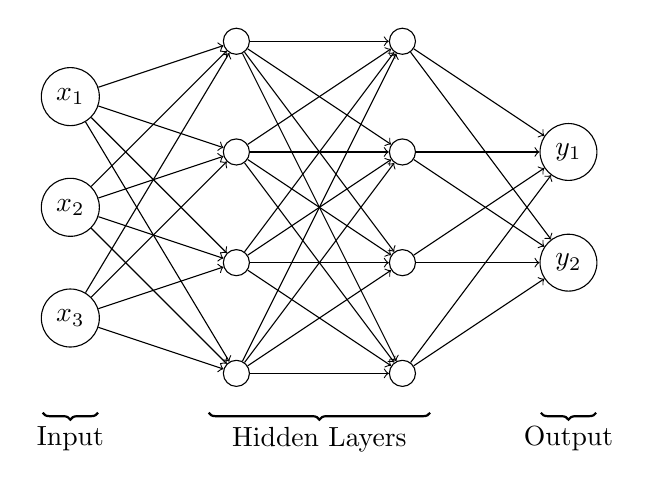
\begin{tikzpicture}[x=1em,y=1em]
  % Input layer
  \foreach \i in {1,...,3}{
    \node[draw, circle] (N-1-\i) at (0, 10 + 4 - 4 * \i) {$x_{\i}$};
  }
  % Hidden layer 1
  \foreach \i in {1,...,4}{
    \node[draw, circle] (N-2-\i) at (6, 12 + 4 - 4 * \i) {};
    \foreach \j in {1,...,3}{
      \draw [->] (N-1-\j) -- (N-2-\i);
    }
  }
  % Hidden layer 2
  \foreach \i in {1,...,4}{
    \node[draw, circle] (N-3-\i) at (12, 12 + 4 - 4 * \i) {};
    \foreach \j in {1,...,4}{
      \draw [->] (N-2-\j) -- (N-3-\i);
    }
  }
  % Output layer
  \foreach \i in {1,...,2}{
    \node[draw, circle] (N-4-\i) at (18, 8 + 4 - 4 * \i) {$y_{\i}$};
    \foreach \j in {1,...,4}{
      \draw [->] (N-3-\j) -- (N-4-\i);
    }
  }
\draw [thick, decoration={brace, mirror, raise=0.5cm}, decorate] (-1,0) -- (1,0) node[pos=0.5,anchor=north,yshift=-0.55cm] {Input};
\draw [thick, decoration={brace, mirror, raise=0.5cm}, decorate] (5,0) -- (13,0) node[pos=0.5,anchor=north,yshift=-0.55cm] {Hidden Layers};
\draw [thick, decoration={brace, mirror, raise=0.5cm}, decorate] (17,0) -- (19,0) node[pos=0.5,anchor=north,yshift=-0.55cm] {Output};
\end{tikzpicture}
\unskip}
  \caption{Feed-forward neural network with input dimension 3, output dimension 2 and 2 hidden layers of dimension 4 each.}
  \label{fig:ae}
\end{figure}

\subsubsection{Basic Principles}
\newpage \phantom{x}
\newpage

\subsubsection{Learning in Artificial Neural Networks}

History of backprop (citations like/leading to \cite{nature_backprop}). SGD, Momentum, ... second order methods?

\newpage \phantom{x}
\newpage

\subsubsection{Modern Advances and Best Practices}
\newpage \phantom{x}
\newpage

\subsection{Autoencoders}
\label{subsection:autoencoders}

\begin{figure}[!htb]
  \centering
  \resizebox{\textwidth}{!}{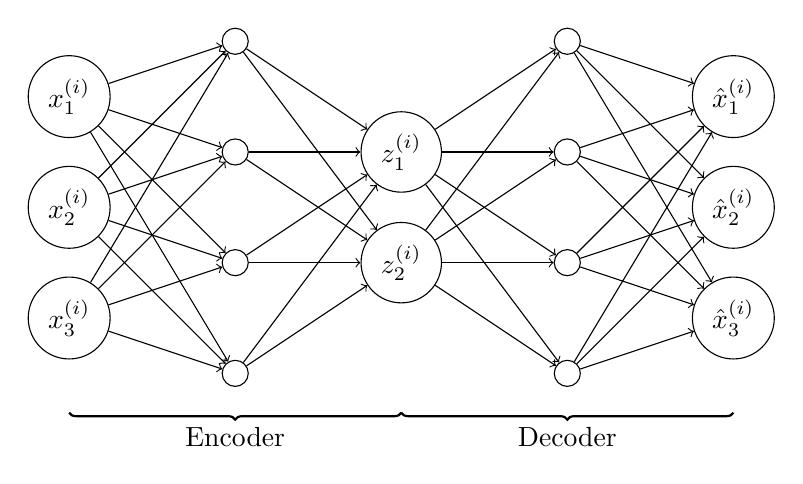
\begin{tikzpicture}[x=1em,y=1em]
  % Input layer
  \foreach \i in {1,...,3}{
    \node[draw, circle] (N-1-\i) at (0, 10 + 4 - 4 * \i) {$x^{(i)}_{\i}$};
  }
  % Encoder hidden layer
  \foreach \i in {1,...,4}{
    \node[draw, circle] (N-2-\i) at (6, 12 + 4 - 4 * \i) {};
    \foreach \j in {1,...,3}{
      \draw [->] (N-1-\j) -- (N-2-\i);
    }
  }
  % Latent code
  \foreach \i in {1,...,2}{
    \node[draw, circle] (N-3-\i) at (12, 8 + 4 - 4 * \i) {$z^{(i)}_{\i}$};
    \foreach \j in {1,...,4}{
      \draw [->] (N-2-\j) -- (N-3-\i);
    }
  }
  % Decoder hidden layer
  \foreach \i in {1,...,4}{
    \node[draw, circle] (N-4-\i) at (18, 12 + 4 - 4 * \i) {};
    \foreach \j in {1,...,2}{
      \draw [->] (N-3-\j) -- (N-4-\i);
    }
  }
  % Output layer
  \foreach \i in {1,...,3}{
    \node[draw, circle] (N-5-\i) at (24, 10 + 4 - 4 * \i) {$\hat{x}^{(i)}_{\i}$};
    \foreach \j in {1,...,4}{
      \draw [->] (N-4-\j) -- (N-5-\i);
    }
  }
\draw [thick, decoration={brace, mirror, raise=0.5cm}, decorate] (0,0) -- (12,0) node[pos=0.5,anchor=north,yshift=-0.55cm] {Encoder};
\draw [thick, decoration={brace, mirror, raise=0.5cm}, decorate] (12,0) -- (24,0) node[pos=0.5,anchor=north,yshift=-0.55cm] {Decoder};
\end{tikzpicture}
\unskip}
  \caption{Autoencoder}
  \label{fig:ae}
\end{figure}

\newpage \phantom{x}
\newpage

\subsection{Variational Bayesian Methods}
\label{subsection:variational_inference}

\subsubsection{Kullback-Leibler Divergence}

The Kullback-Leibler divergence, or KL-divergence for short, is a measure of dissimilarity between two probability distributions.

For continuous probability distributions $p$ and $q$ the Kullback-Leibler divergence is defined as

$$\dkl{p}{q} = \int p(\mathbf{x}) \log \frac{p(\mathbf{x})}{q(\mathbf{x})} d\mathbf{x},$$

and likewise for discrete probability distributions as

$$\dkl{p}{q} = \sum_{i} p(i) \log \frac{p(i)}{q(i)}.$$

The following properties hold for 

One must note however that KL-divergence is asymmetric, i.e. $\dkl{p}{q} \neq \dkl{q}{p}$, and thus cannot readily be used as a metric.

\subsubsection{The Evidence Lower Bound}

\newpage

\subsection{Auto Encoding Variational Bayes}

\begin{figure}[!htb]
  \centering
  \resizebox{\textwidth}{!}{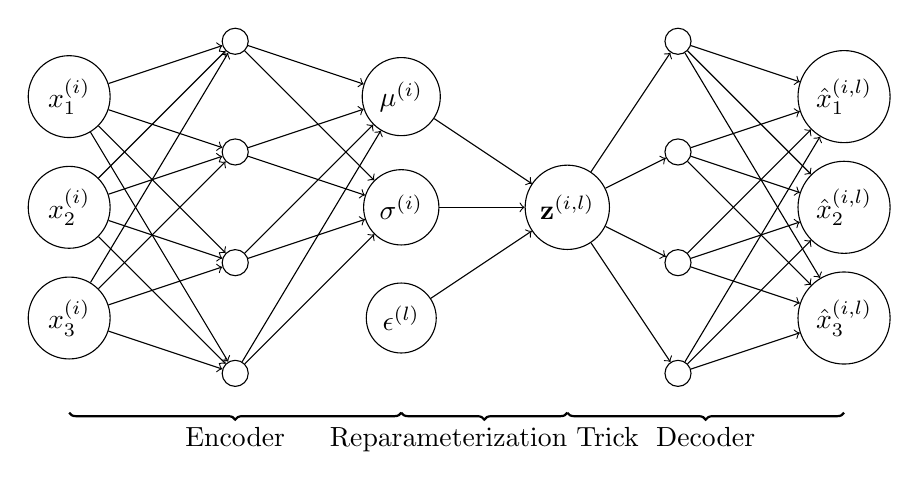
\begin{tikzpicture}[x=1em,y=1em]
  % Input layer
  \foreach \i in {1,...,3}{
    \node[draw, circle] (N-1-\i) at (0, 10 + 4 - 4 * \i) {$x^{(i)}_{\i}$};
  }
  % Encoder hidden layer
  \foreach \i in {1,...,4}{
    \node[draw, circle] (N-2-\i) at (6, 12 + 4 - 4 * \i) {};
    \foreach \j in {1,...,3}{
      \draw [->] (N-1-\j) -- (N-2-\i);
    }
  }
  % Latent code
  \node[draw, circle] (mu) at (12, 10) {$\mathbf{\mu}^{(i)}$};
  \node[draw, circle] (sigma) at (12, 6) {$\mathbf{\sigma}^{(i)}$};
  \node[draw, circle] (eps) at (12, 2) {$\mathbf{\epsilon}^{(l)}$};
  \node[draw, circle] (z) at (18, 6) {$\mathbf{z}^{(i, l)}$};
  \foreach \x in {mu,sigma,eps}{
    \draw [->] (\x) -- (z);
  }
  \foreach \x in {mu,sigma}{
    \foreach \j in {1,...,4}{
      \draw [->] (N-2-\j) -- (\x);
    }
  }
  % Decoder hidden layer
  \foreach \i in {1,...,4}{
    \node[draw, circle] (N-4-\i) at (22, 12 + 4 - 4 * \i) {};
    \draw [->] (z) -- (N-4-\i);
  }
  % Output layer
  \foreach \i in {1,...,3}{
    \node[draw, circle] (N-5-\i) at (28, 10 + 4 - 4 * \i) {$\hat{x}^{(i, l)}_{\i}$};
    \foreach \j in {1,...,4}{
      \draw [->] (N-4-\j) -- (N-5-\i);
    }
  }
  \draw [thick, decoration={brace, mirror, raise=0.5cm}, decorate] (0,0) -- (12,0) node[pos=0.5,anchor=north,yshift=-0.55cm] {Encoder};
  \draw [thick, decoration={brace, mirror, raise=0.5cm}, decorate] (12,0) -- (18,0) node[pos=0.5,anchor=north,yshift=-0.55cm] {Reparameterization Trick};
  \draw [thick, decoration={brace, mirror, raise=0.5cm}, decorate] (18,0) -- (28,0) node[pos=0.5,anchor=north,yshift=-0.55cm] {Decoder};
\end{tikzpicture}
\unskip}
  \caption{Variational Autoencoder}
  \label{fig:vae}
\end{figure}

\begin{figure}[!htb]
  \centering
  \resizebox{0.3\textwidth}{!}{\begin{tikzpicture}
  \node[obs]                (x) {$\mathbf{x}$};
  \node[latent, left=of x]  (z) {$\mathbf{z}$};
  \node[latent, above=of x] (t) {$\mathbf{\theta}$};
  \node[latent, above=of z] (p) {$\mathbf{\phi}$};
  
  \edge[bend left]          {z} {x};
  \edge[bend left, dashed]  {x} {z};
  \edge                     {t} {z};
  \edge                     {t} {x};
  \edge[dashed]             {p} {z};
  
  \plate {zx} {(x)(z)}      {$N$};
\end{tikzpicture}
\unskip}
  \caption{AEVB plate notation}
  \label{fig:aevb_plate_notation}
\end{figure}

\newcommand{\ptheta}{p_{\mathbf{\theta}}}
\newcommand{\qphi}{q_{\mathbf{\phi}}}
\newcommand{\bxi}{\mathbf{x}^{(i)}}
\newcommand{\bz}{\mathbf{z}}

\subsubsection{Derivation of the VAE Objective Function}

The objective of VAEs is to model the data as well as possible, i.e. maximize the marginal likelihood $\ptheta(\bxi)$ for each data point $i$. By an application of Jensen's inequality we can derive the following lower bound for the marginal likelihood under our latent variable model:

\begin{equation}
\begin{aligned}
\log \ptheta(\bxi) & = \log \int \ptheta(\bxi \vert \bz) p(\bz) d\bz \\
                   & = \log \int \frac{\qphi(\bz \vert \bxi)}{\qphi(\bz \vert \bxi)} \ptheta(\bxi \vert \bz) p(\bz) d\bz \\
                   & = \log \mathbb{E}_{\qphi(\bz \vert \bxi)}\Big[\frac{\ptheta(\bxi \vert \bz) p(\bz)}{\qphi(\bz \vert \bxi)}\Big] \\
                   & \geq \mathbb{E}_{\qphi(\bz \vert \bxi)}\Big[\log \frac{p(\bz)}{\qphi(\bz \vert \bxi)}\Big] + \mathbb{E}_{\qphi(\bz \vert \bxi)}\Big[\log \ptheta(\bxi \vert \bz)\Big] \\
                   & = -\dkl{\qphi(\bz \vert \bxi)}{p(\bz)} + \mathbb{E}_{\qphi(\bz \vert \bxi)}\Big[\log \ptheta(\bxi \vert \bz)\Big].
\end{aligned}
\end{equation}

This bound is better known as the \textit{evidence lower bound}, or ELBO for short. An interpretation for the terms of the last equation is that the objective is to have the posterior $\qphi(\bz \vert \bxi)$ match the prior $p(\bz)$ as accurately as 

In many cases the KL-divergence can be integrated analytically, for instance in the case of two Gaussian distributions. In cases where the KL term cannot be solved analytically, Monte Carlo methods are used to approximate the expectation.

Several modifications to this objective have been proposed, e.g. the $\beta$-VAE \cite{beta_vae, understanding_beta_vae}, $\beta$-TCVAE \cite{beta_tcvae} and InfoVAE \cite{infovae}.

\subsubsection{Obtaining Differentiable Monte Carlo Estimates}

To optimize the parameters $\mathbf{\theta}$ and $\mathbf{\phi}$ of our neural network using backpropagation we require a way to compute the gradient of the expectations of random variables. By introducing a random noise variable as input we are able to obtain samples from the latent distribution by using the \textit{reparameterization trick}.

$$\widetilde{\mathbf{z}} = g_{\mathbf{\phi}}(\mathbf{\epsilon}, \mathbf{z})$$

\newpage \phantom{x}
\newpage \phantom{x}
\newpage

\section{t-Distributed Stochastic Neighbor Embedding}
\label{section:tsne}
\subsection{SNE}
\label{subsection:sne}
\newpage

\subsection{t-SNE}
\label{subsection:tsne}

$$2^{H(p(\mathbf{x}))} = 2^{-\sum_{i=1}^{N} p(\mathbf{x}^{(i)}) \log_2 p(\mathbf{x}^{(i)})}$$

$$q_{ij} = \frac{(1 + \mathbf{y}_i - \mathbf{y}_j)^{-1}}{\sum_{k \neq l} (1 + \mathbf{y}_k - \mathbf{y}_l)^{-1}}$$

$$p_{ij} = \frac{p_{j \vert i} + p_{i \vert j}}{2 N}$$

$$C = \dkl{P}{Q} = \sum_i \sum_j p_{ij} \log \frac{p_{ij}}{q_{ij}}$$

$$\frac{\partial C}{\partial \mathbf{y}_i} = $$

\newpage \phantom{x}
\newpage \phantom{x}
\newpage

\subsection{Parametric t-SNE}
\label{subsection:parametric_tsne}
\newpage

\chapter{Method}
\label{ch:method}

\section{Learning a Parametric Embedding Using VAE Sampling}
\newpage \phantom{x}
\newpage \phantom{x}
\newpage

\section{Robustness to Sparse and Noisy Data}
\label{section:robustness_to_sparse_and_noisy_data}
\newpage

\section{Sampling from Hidden Layers}
\label{section:sampling_from_hidden_layers}
\newpage

\section{Inference with the Generative Model}
\newpage

\section{Implementation}
\label{section:implementation}

An accompanying implementation of the method has been made available at \url{https://github.com/ahie/vptsne}. The implementation is built on top of Tensorflow \citep{tensorflow} and takes advantage of the Tensorflow Distributions \citep{tensorflow_distributions} library. To take full advantage of the computation graph architecture of Tensorflow and the paralellism provided by GPGPUs, both the t-SNE loss and its gradient computation were implemented as custom CUDA \citep{cuda} kernel operations.

\note{Describe that it also includes fast parallel implementation of NN-Descent \citep{nn_descent}?}

\chapter{Experiments}
\label{ch:experiments}

The code and data used to reproduce all the results presented in this section have been made available at \url{https://github.com/ahie/vptsne-results}.

\section{Data Sets}
\label{subsection:data_sets}

To validate the proposed method we studied the properties of the combined model on the four different data sets described below.

\subsection{MNIST}
\label{subsubsection:mnist}

The MNIST data set \citep{mnist} contains labeled images of handwritten digits. Each image contains a single digit in gray-scale with a resolution of 28x28 pixels. The data set is split into $60000$ training images and $10000$ test images. All networks were trained solely on the training data set, while the remaining test examples were reserved for assessing the capability of the network to generalize to out-of-sample extensions. In the unsupervised setting considered here, the provided labels were only used for visualizing the embeddings and evaluating the embedding quality of out-of-sample extensions via an 1-NN classifier.

\subsection{Fashion-MNIST}
\label{subsubsection:fashion_mnist}

\textcolor{red}{Move to supplement? Currently only used in section \ref{subsection:learning}. Ref. \citep{fashion_mnist}}

\subsection{Mass Cytometry}
\label{subsubsection:mass_cytometry}

Cytometry is the measurement of biological characteristics of cells. In mass cytometry time-of-flight mass spectrometry is used to measure the counts of cellular proteins present within a single cell by tagging proteins with their corresponding antibodies that have been conjugated with specific heavy metals.

As a comparatively new methodological development, mass cytometry enables simultaneous measurement of a considerably greater number of features compared to fluorescence based flow cytometry. A greater number of features however poses new challenges in analyzing the measurement results. To aid the analysis of this high dimensional data it is common to visualize the data as a 2-D or 3-D scatter plot using t-SNE, due to its capability to separate biologically relevant subpopulations of cells in the produced embedding \citep{visne}. However, as a high-throughput method, mass cytometry data sets under analysis can grow to be millions of data points in size, prompting the use of more scalable algorithms. For a more thorough review on mass cytometry and associated analytical challenges the reader is referred to \cite{mass_cytometry}.

In our experiments we consider two different mass cytometry data sets. As the first data set, henceforth referred to as Cytometry A, we use the publicly available data of \cite{phenograph}, which has been used to demonstrate the effectiveness of the Phenograph clustering algorithm on mass cytometry data. The data set consists of $81000$ data points of $13$ dimensions corresponding to the normalized counts of cell surface proteins belonging to distinct clusters of differentiation. As a benchmark data set for the Phenograph clustering algorithm we additionally include the labels produced by Phenograph in our analysis.

The second mass cytometry data set (Cytometry B) contains data gathered from ovarian cancer patients at different phases of treatment. The number of points in the entire data set is $1.4$ million, each of which has $23$ dimensions.

\newpage
\section{Evaluation Metrics}
\subsection{Nearest Neighbor Classifier}
\subsection{Trustworthiness}
\newpage

\section{Network Structure and Parameters}
\label{subsection:network_structure_and_parameters}

To parameterize the embedding $f(\mathbf{\hat{x}})$ a feed-forward neural network with layers of hidden units with dimensions $d \times 28 - 500 - 500 - 2000 - 2$ were used, where $d$ is the input dimensionality and rectifier linear unit (ReLU) activations are applied to the hidden unit outputs to induce nonlinearity to the network. The hidden unit dimensions were chosen to match those of the final combined network used in \citep{parametric_tsne}, although we have substituted the sigmoid activations with ReLU activations. Furthermore, we do not perform stacked restricted Boltzmann machine pretraining on the hidden layer weigths as in \citep{parametric_tsne}. However we do benchmark the performance of our network against the original parametric t-SNE implementation. Since we are not considering RBM pretraining and are instead relying on the property of ReLUs reducing the vanishing gradient problem \citep{relu} and better initialization \citep{xavier_initializer}. Running the original implementation shows little benefit in performing this costly initialization. We could instead reuse the trained encoder weights of the VAE as a starting point for the optimization of our embedding network.

For optimization of the neural network \cite{parametric_tsne} use nonlinear conjugate gradient descent, whereas Adam \citep{adam} is used as the optimizer in our results. Updates with Adam are considerably faster to compute than with conjugate gradient descent. Throughout all experiments standard parameters for Adam were chosen, i.e. a learning rate of $0.001$ and the exponential decay rates of the 1st and 2nd moments were set to $0.9$ and $0.999$ respectively.

\textcolor{red}{[Note: Should mention recent work on Adam, i.e. the updated version by \cite{on_the_convergence_of_adam}?]}

We apply batch normalization \citep{batch_normalization} to the hidden layers of the VAE networks, while omitting batch normalization from the embedding network. This is to validate the training procedure on as simple an embedding network as possible. We note that applying batch normalization to the embedding network improves the results marginally.

To further emphasize the universality of our approach we restrict ourselves to use a simple VAE structure, without complicating the model architecture with more recently proposed advances, such as normalizing flows \citep{normalizing_flows} (\textcolor{red}{[Note: could show that better models improve performance in the supplement]}). Throughout all experiments the VAE architecture is fixed to $d - 256 - 128 - 32 - \mu, \log \sigma^2 - 32 - 128 - 256 - d$, where $\mu$ and $\sigma$ parameterize a normal distribution acting as the posterior $q_{\phi}(\mathbf{z} \vert \mathbf{x}^{(i)})$ and the final layer output was used to parameterize a Bernoulli distribution for MNIST as well as Fashion-MNIST, and a normal distribution with a fixed standard deviation of 0.1 for cytometry data. In all experiments, each VAE was trained with a batch size of 1000 for 10000 iterations.

The perplexities used for each data set were chosen such that the trained embeddings produced the best results. For MNIST and Fashion-MNIST perplexities were set to 30, which is in line with the value used by \cite{parametric_tsne}, whereas for the cytometry data sets a perplexity of 10 was chosen.

\section{Learning}
\label{subsection:learning}

In this section we compare the effect of training on VAE reconstructions to training on the original MNIST data set. To quantitatively evaluate the quality of the embeddings produced we employed the trustworthiness metric \citep{trustworthiness} on the MNIST test set. Additionally, we compared the 1-NN classification errors by fitting the classifiers on the produced embeddings of the training set and finding the mean accuracies of the classifiers on the test set.

In figure \ref{fig:mnist_knn_trustworthiness} we have plotted the 1-NN scores and trustworthiness of the embeddings obtained after each iteration of training for two different batch sizes. The runs for each batch size were repeated 20 times, plotting the means and 95\% confidence intervals. Training with VAE reconstructions shows a clear improvement both qualitatively and quantitatively over training on the original data when small training batches are used to approximate the t-SNE loss gradient. Higher trustworthiness, as well as 1-NN scores are obtained consistently and convergence is reached with far fewer iterations. Moreover, the results are in favor of training on reconstructions by exhibiting more stable results during training.

Qualitatively the embeddings trained on the original data remain noisier than the embeddings trained on the reconstructed data points. This can be seen in figure \ref{fig:mnist_comparison}, where the separation of true clusters in the embedding is far less evident, with several classes overlapping and a large number of outlier points for each class. We further compare the qualitative differences of the embeddings produced with the Fashion-MNIST dataset. In figure \ref{fig:fashion_mnist_comparison} similar deficiencies in the embedding can be noted as in the embedding comparisons for the MNIST data set. In particular, the visible clusters of classes are less distinct, as well as the global layout of the classes is considerably worse, e.g. the cluster of footwear related images has been pulled closer to the cluster of upper body garments and the images of bags have been split into two seemingly unrelated clusters.

\begin{figure}[!htb]
  \centering
  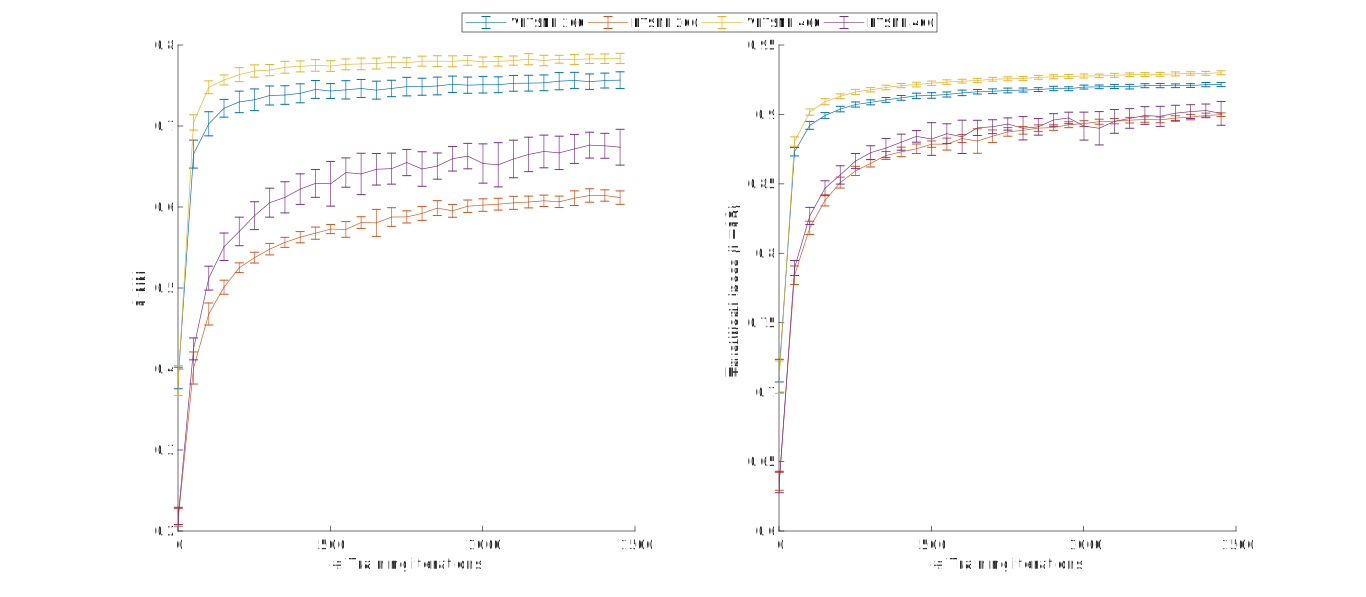
\includegraphics[width=\textwidth]{images/learning_curves.png}
  \caption{Plots of 1-NN and trustworthiness scores obtained after a given number of iterations for different batch sizes. The means and 95\% confidence intervals have been plotted from 20 repeated runs for each parameter setting.}
  \label{fig:mnist_knn_trustworthiness}
\end{figure}

\begin{figure}[!htb]
  \centering
  \begin{tabular}{cc}
    \includegraphics[width=0.45\textwidth]{images/mnist_ptsne_embedding.png} &
    \includegraphics[width=0.45\textwidth]{images/mnist_vptsne_embedding.png} \\
    \multicolumn{2}{c}{\includegraphics[width=0.45\textwidth]{images/mnist_legend.png}}
  \end{tabular}
  \caption{Embeddings of the MNIST data set trained with batch size 400.}
  \label{fig:mnist_comparison}
\end{figure}

\begin{figure}[!htb]
  \centering
  \begin{tabular}{cc}
    \includegraphics[width=0.45\textwidth]{images/fashion_mnist_ptsne_embedding.png} &
    \includegraphics[width=0.45\textwidth]{images/fashion_mnist_vptsne_embedding.png} \\
    \multicolumn{2}{c}{\includegraphics[width=0.45\textwidth]{images/fashion_mnist_legend.png}}
  \end{tabular}
  \caption{Embeddings of the Fashion-MNIST data set trained with batch size 400. \textcolor{red}{[Note: could include UMAP embedding of this data set here for comparison. It is very similar and this would reinforce the claim that small batch size training is actually very effective.]}}
  \label{fig:fashion_mnist_comparison}
\end{figure}

\textcolor{red}{??? Plot like Figure~\ref{fig:mnist_knn_trustworthiness} for VPTSNE vs PTSNE with batch size on x to show that VPTSNE does not suffer that much from small batch sizes? This would imply that it can be trained with smaller batch sizes, which means better asymptotic performance. ???} 

\section{Comparisons}
\label{subsection:comparisons}

We now compare the proposed method to other parametric dimensionality reduction methods, namely PCA, VAE and Autoencoders. In addition we also consider two non-parametric dimensionality reduction methods, t-SNE and the recently proposed method UMAP \citep{umap}, which had been demonstrated to be able to produce embeddings comparable to t-SNE while being more efficient to optimize in practice.

For the comparisons we will be using the Cytometry A data set. As evaluation criteria, similarly to the previous section, both trustworthiness and 1-NN classification accuracy are used. In addition to comparing the quality of the embeddings, the runtime performance of the different methods are studied. Our goal is to demonstrate that our method produces competitive embeddings as well as has superior scalability.

\subsection{Embedding Quality}
\label{subsubsection:embedding_quality}

The quantitative results for all methods under comparison are available in table \ref{table:comparison} and the corresponding scatter plots of the 2-D embeddings are presented in figure \ref{fig:comparison_figure}. Although VAE produces quantitatively better results for the chosen metrics, the spatial layout of clusters in the resulting embedding have less distinct separation and the global structure of the embedding is constrained by the chosen prior $p(\mathbf{z})$. From a data visualization standpoint these factors make the latent space embeddings qualitatively worse than what the corresponding quantitative metrics would suggest. Unsurprisingly, PCA performs the worst on both quantitative and qualitative results. Our method however is able to reach results on par with those of the chosen non-parametric methods.

\textcolor{red}{[Note: Should find/develop some metric for comparing how well global structure is preserved?]}

\subsection{Scalability}
\label{subsubsection:scalability}

A major practical challenge with nonlinear dimensionality reduction methods are their scalability to large data sets. Typically, to capture the spatial structure of data a distance metric is employed to compute the pairwise distances for the entire data set, after which a projection of the points to a lower dimensional space, equipped with a corresponding metric, is sought that retains the computed distances as accurately as possible. As the number of data points increases, the inherent quadratic complexity of methods relying on such pairwise distance computations quickly renders such methods intractable.

\textcolor{red}{In practice, with small batch sizes direct computation of the t-SNE gradient outperforms the use of auxiliary data structures such as the Barnes-Hut approximation introduced in \citep{accelerated_tsne_2}. While direct computation of the gradient is asymptotically bounded by $\mathcal{O}(k^2)$, where $k$ is the chosen batch size, the operations needed to be carried out for its computation can be efficiently performed in parallel}. Choosing a $k$ for which $k \ll n$ and the smaller batch size retains adequate information about the underlying data distribution is at the heart of the considerable runtime advantage our method has over those under comparison.

To demonstrate the real world performance of our proposed method the wall clock times taken by each algorithm to produce embeddings for subsets of the Cytometry B data set have been plotted in figure \textcolor{red}{[add the figure]}. \textcolor{red}{[verify the next sentence (preliminary results do show good performance)]} The empirical results presented in the figure show significant performance gains, even for smaller data set sizes, over the other algorithms under consideration.

\textcolor{red}{
\begin{itemize}
\item Even with the Barnes-Hut approximation t-SNE is far less scalable in practice. This occurs when a large number of points are in close proximity and the interactions can't be approximated efficiently.
\item Optimizing UMAP can be done via approximating stochastically its gradient via edge sampling, this is the key to its performance. Inspired by \citep{largevis}, where dimensionality reduction is done by laying out a graph with the SNE $P_{ij}$ matrix as its adjacency matrix.
\item 
\end{itemize}
}

\begin{table}[]
\centering
\caption{Comparison between different dimensionality reduction methods.}
\label{table:comparison}
\begin{tabular}{cccc}
Algorithm   & Trustworthiness ($k=12$)   & 1-NN     & time (ms) \\ \hline \hline
VPTSNE      & $0.9753$                   & $0.9250$ & $60766$   \\ \hline
PTSNE       & $0.9628$                   & $0.8890$ & $8729$    \\ \hline
VAE         & $0.9762$                   & $0.9247$ & $52037$   \\ \hline
PCA         & $0.8557$                   & $0.4886$ & $96$      \\ \hline
UMAP        & $0.9688$                   & $0.9297$ & $74716$   \\ \hline
t-SNE       & $0.9879$                   & $0.9536$ & $1192812$ \\ \hline
\end{tabular}
\end{table}

\begin{figure}[!htb]
  \centering
  \begin{tabular}{cccc}
    VPTSNE &
    \raisebox{-.5\height}{\includegraphics[width=0.25\textwidth]{images/vptsne_levine.png}} &
    \raisebox{-.5\height}{\includegraphics[width=0.25\textwidth]{images/vptsne_levine_zoomed.png}} &
    \raisebox{-.5\height}{\includegraphics[width=0.25\textwidth]{images/vptsne_levine_zoomed_2.png}} \\
    UMAP &
    \raisebox{-.5\height}{\includegraphics[width=0.25\textwidth]{images/umap_levine.png}} &
    \raisebox{-.5\height}{\includegraphics[width=0.25\textwidth]{images/umap_levine_zoomed.png}} &
    \raisebox{-.5\height}{\includegraphics[width=0.25\textwidth]{images/umap_levine_zoomed_2.png}} \\
    VAE &
    \raisebox{-.5\height}{\includegraphics[width=0.25\textwidth]{images/vae_levine.png}} &
    \raisebox{-.5\height}{\includegraphics[width=0.25\textwidth]{images/vae_levine_zoomed.png}} &
    \raisebox{-.5\height}{\includegraphics[width=0.25\textwidth]{images/vae_levine_zoomed_2.png}} \\
  \end{tabular}
  \caption{Cytometry A data set embedded with the methods being compared in section \ref{subsection:comparisons}. \textcolor{red}{[Note: Add the rest, currently missing PTSNE, PCA, t-SNE.]}}
  \label{fig:comparison_figure}
\end{figure}

\section{Robustness to Sparse Data}
\label{subsection:robustness_to_sparse_data}

As discussed in section \textcolor{red}{[ref. the correct section]} the probabilistic model is advantageous when only few data points are available. To show this effect in practice we trained mappings with and without the use of our method on random 0.01\% subsets of the MNIST data set. As the size of the subsets were only 600 data points each, we were able to use batch gradient descent while training the PTSNE mapping. For training VPTSNE we took advantage of the probabilistic model by sampling data points from the posterior distributions of the training data points, effectively creating different batches of 600 data points at each iteration. Evaluation of the mappings was carried out on the full MNIST test set as in previous experiments. The experiment was repeated 20 times on different subsets. Boxplots corresponding to the obtained scores can be found in figure \ref{fig:subset_combined_boxplot}. Significant differences in the obtained scores are noted in favor of our method (one-tailed t-test: 1-NN $p=6.1309E-08$, trustworthiness $p=9.9365E-05$). From these results we can observe that both the trustworthiness and 1-NN scores remain higher even with extremely small data sets, indicating that the use of our method is able to provide better generalization even when few training data points are available.

\begin{figure}[!htb]
  \centering
  \includegraphics[width=\textwidth]{images/subset_combined_boxplot.png}
  \caption{Boxplots of 1-NN and trustworthiness scores obtained for PTSNE and VPTSNE trained on 0.01\% subsets of the MNIST data set.}
  \label{fig:subset_combined_boxplot}
\end{figure}

\textcolor{red}{ A plot with sparsity (downsampling factor on x, and goodness on y, like we had previously }  

\section{Robustness to Noisy Data}
\label{subsection:robustness_to_noisy_data}

As real world data is generally not perfectly clean, an important property for any machine learning method is its capability to handle data containing artefacts. Considering VAEs are inherently robust to corrupted data due to the regularization provided by the stochastic latent code (\textcolor{red}{[should be discussed in a previous section more thoroughly, connection with VAE and RPCA \citep{rpca_1, rpca_2} shown in \citep{hidden_talents_of_the_vae}]}) it is reasonable to assume that a training procedure for a low dimensional mapping taking advantage of this property would perform better on corrupted data than one that is subjected only to the raw data.

Here we aim to back up this assumption by running experiments on artificially corrupted MNIST data sets. As the corruption process in our experiments we consider \textit{masking noise} as in \cite{stacked_denoising_ae}, where a predetermined fraction of randomly chosen elements of a data point are set to 0. We test robustness by applying masking noise to 20\% and 30\% fractions of the training set. Following training we test generalization on the uncorrupted test set.

The results of our experiments (see figure \ref{fig:corrupted_data}) show a clear advantage to using our method when dealing with noisy data as both evaluation metrics can be observed to decrease considerably for PTSNE as the training data is progressively corrupted, whereas VPTSNE maintains its performance throughout the experiments.

\noindent \textcolor{red}{[Note: Results look good, but could they be further improved by denoising variational autoencoders \citep{denoising_vae}?]}

\noindent \textcolor{red}{[Note: In scRNA-seq dropout events can be viewed as masking noise. The results here would indicate applying the method to scRNA-seq data could produce good results.]}

\noindent \textcolor{red}{[Note: Should other corruption processes be considered here or is masking noise sufficient?]}

\noindent \textcolor{red}{[Note: Could add scatter plot of the best scoring embeddings PTSNE vs VPTSNE to the supplement for e.g. the 30\% corrupted runs. The difference is quite striking.]}

\begin{figure}[!htb]
  \centering
  \includegraphics[width=\textwidth]{images/corrupted_data.png}
  \caption{Boxplots of 1-NN and trustworthiness scores obtained for PTSNE and VPTSNE trained on MNIST data with different levels of masking noise applied. \textcolor{red}{Change to line plot with confidence intervals once more test runs are completed for different corruption \%.}}
  \label{fig:corrupted_data}
\end{figure}

\textcolor{red}{ Again, I would want more points on the graphs. Noise level on x axis and score on y. }

\section{Sampling from Hidden Layers}
\label{subsection:obtaining_reconstructions_from_hidden_layers}

\textcolor{red}{[Note: Much of this will probably be moved to the methods section.]}

Instead of training the embedding network on the final output of the observation model it is possible to instead use the outputs of a chosen hidden layer. If the chosen hidden layer has dimensions $d_{hidden} \ll d_{input}$ the benefits of this approach are twofold:

\begin{itemize}
\item We are performing a step of nonlinear dimensionality reduction that is not dependent on local distance metrics, i.e. a preprocessing step that is less susceptible to the \textit{curse of dimensionality}.
\item Given that the number of dimensions can be chosen to be considerably lower than in the original input space, computing the t-SNE loss also becomes proportionally cheaper.
\end{itemize}

To show the efficacy of this modification to the learning procedure we train an embedding using the latent code directly. As we choose the dimensionality of the latent code to be more than two orders of magnitude smaller than that of the original data's it is possible for us to use batches of far greater size to train the embedding network, without incurring additional computation cost over training with smaller batches on data of the original dimensionality. The latent dimensionality of the VAE was chosen to be $7$ and the batch size for training the embedding was set to $5000$, as in the original parametric t-SNE paper by \cite{parametric_tsne}. We have additionally included the embedding of data points obtained with the original implementation of parametric t-SNE for comparison in figure \ref{fig:hidden_layer}. Qualitatively \textcolor{red}{and quantitatively ([still WIP])} we achieve an overall better embedding with less computation using our method.

When considering precomputed $P_{ij}$ matrices for each batch the gain in computational advantage does however diminish significantly, although the following caveats apply to the precomputation: Storing the precomputed matrices will require considerable space for large batch sizes and data sets. A way to circumvent the need for large storage space is to employ the KNN approximation introduced in \citep{accelerated_tsne_2} when computing $P_{ij}$, i.e. only considering a small number of neighbors when computing the conditional probabilities for each pair of points, which will result in a sparse matrix. This however increases the error in the computed gradient and relies on an efficient KNN algorithm in practice. Additionally, fixing the batches in advance hinders the performance of SGD as the gradient estimates become biased. Moreover, relying on precomputed $P_{ij}$ matrices for fixed batches prevents the use of infinite sample generation from the VAE.

\begin{figure}[!htb]
  \centering
  \includegraphics[width=\textwidth]{images/vptsne_vs_original_ptsne_7.png}
  \caption{Embedding produced by training on a 7 dimensional latent representation of the MNIST data set contrasted with the original implementation of \cite{parametric_tsne} run on the original data.}
  \label{fig:hidden_layer}
\end{figure}

\textcolor{red}{[Note: The choice of 7 as the latent dimensionality right now seems unjustified. It was simply chosen to be the largest number for which "more than two orders of magnitude smaller" holds true. Should work that into the text.]}

\section{Inference with the Generative Model}
\label{subsection:applications_of_the_inference_network}

From the underlying generative model we can approximately compute the marginal $p(\mathbf{x}^{(i)})$ for each data point $\mathbf{x}^{(i)}$. An approximation can be retrieved by importance sampling \citep{stochastic_backpropagation}:

$$p(\mathbf{x}) \approx \frac{1}{N} \sum_{i=1}^{N} \frac{p(\mathbf{x} \vert \mathbf{z}^{(i)}) p(\mathbf{z}^{(i)})}{q_{\theta}(\mathbf{z}^{(i)} \vert \mathbf{x})},$$

where $\mathbf{z}^{(i)} \sim q_{\theta}(\mathbf{z} \vert \mathbf{x})$.

Using the obtained marginals as feedback we can inform the user of potentially anomalous points in the data set. This feedback can then further be used in downstream analysis. From a data visualization perspective points that do not fit the model well correspond to points that are likely to be mapped poorly, thus removing such outliers from the final mapping serves to highlight the natural clusters in the data more clearly.

\textcolor{red}{[Note: discuss the more accurate but computationally costly marginal estimation method: annealed importance sampling \citep{ais, ais_vae}?]}

\textcolor{red}{[Note: could discuss, experiment with modification to the algorithm: if p(x) (or even more simply just the reconstruction error) is high (above some threshold), pass the original data point and not the reconstruction to the mapping. This proved to work for the small subset experiment when limiting the latent dimension to $\leq 3$. Reason for this being that the VAE trained on only 600 samples poorly reconstructed the test set (basically just corrupting many of them).]}

\textcolor{red}{[Note: contents above should be moved to the methods section.]}

As an example we use the Cytometry B data set to train our combined model with two patients' data held out. The protein expression profile of Patient A's cells closely match that of other patients' in the training set, whereas Patient B's sample is from advanced cancer making it an outlier in relation to the data available during training.

To distinguish between outlier and inlier points in the mapping we obtain we set a hard threshold of $\log p(\mathbf{x}) \leq -150$ to separate between the two. In figure \ref{fig:cytometry_outliers} embeddings with both patient specific labeling and labeling obtained by thresholding are shown side by side. The high tumor purity sample of Patient B has almost completely been mapped to a small region corresponding to protein expression levels of cancer cells, whereas Patient A's mapping contains several distinct clusters of various cell types. Further, the labels obtained through thresholding indicate that the majority of cells in Patient B's sample are indeed considered as outliers by the model, in addition to a handful of visually poorly mapped points.

\begin{figure}[!htb]
  \centering
  \begin{tabular}{c}
    \includegraphics[width=\textwidth]{images/scored.png} \\
    \includegraphics[width=\textwidth]{images/scored_zoomed.png}
  \end{tabular}
  \caption{Detecting outliers in cytometry data. \textcolor{red}{[Rename patients to match text.]}}
  \label{fig:cytometry_outliers}
\end{figure}

\chapter{Conclusions}
\label{ch:conclusions}

